\chapter{Relación de Artin}
\label{ch::capitulo2}

\section{Notación de Artin y generadores \(\sigma_i\)}

Para describir una trenza de manera algebraica, consideremos una serie de hilos paralelos, numerados consecutivamente como \(1, 2, 3, \dots, n\). Nuestro objetivo es representar cada cruce entre hilos utilizando una notación que permita describir con precisión la disposición y el entrelazado de los mismos. La notación de Artin introduce los símbolos \(\sigma_i\), que representan un cruce específico entre dos hilos consecutivos.

\subsection{Definiciones}
\subsubsection*{Definición de \(\sigma_i\)}

El generador \(\sigma_i\) representa un cruce en el cual el hilo en la posición \(i\) pasa \textbf{por encima} del hilo en la posición \(i+1\). Cabe destacar que este cruce afecta exclusivamente a estos dos hilos, mientras que los demás permanecen sin alteraciones en sus posiciones.

La interpretación de \(\sigma_i\) es la siguiente:

\begin{itemize}
    \item Al aplicar \(\sigma_i\), el hilo \(i\) se posiciona sobre el hilo \(i+1\), estableciendo un cruce en el cual \(i\) pasa por encima de \(i+1\).
    \item Este cruce representa una operación local entre los hilos \(i\) e \(i+1\), sin afectar la disposición de los demás hilos.
\end{itemize}

Ejemplos específicos incluyen:
\begin{itemize}
    \item \(\sigma_1\): representa el cruce en el cual el primer hilo pasa por encima del segundo.
    \item \(\sigma_2\): indica el cruce donde el segundo hilo pasa por encima del tercero.
\end{itemize}

\subsubsection*{Definición de \(\sigma_i^{-1}\)}

De manera análoga, \(\sigma_i^{-1}\) denota el cruce inverso al de \(\sigma_i\), donde el hilo \(i\) pasa \textbf{por debajo} del hilo \(i+1\). Visualmente, este cruce es el opuesto a \(\sigma_i\) y representa una interacción en la cual el hilo \(i\) se sitúa por debajo del hilo \(i+1\).

\subsection{Construcción de trenzas usando \(\sigma_i\)}

La notación de Artin nos permite representar cualquier trenza compleja como una combinación de generadores \(\sigma_i\) y sus inversos \(\sigma_i^{-1}\). Cada \(\sigma_i\) representa un cruce entre hilos consecutivos, en el cual el hilo \(i\) pasa por encima del hilo \(i+1\), mientras que \(\sigma_i^{-1}\) indica el cruce inverso, donde el hilo \(i\) pasa por debajo del hilo \(i+1\). De esta manera, es posible describir y construir trenzas de cualquier configuración mediante secuencias de estos generadores.

\subsubsection*{Ejemplo de construcción de una trenza compleja}

\begin{figure}[h!]
    \centering
    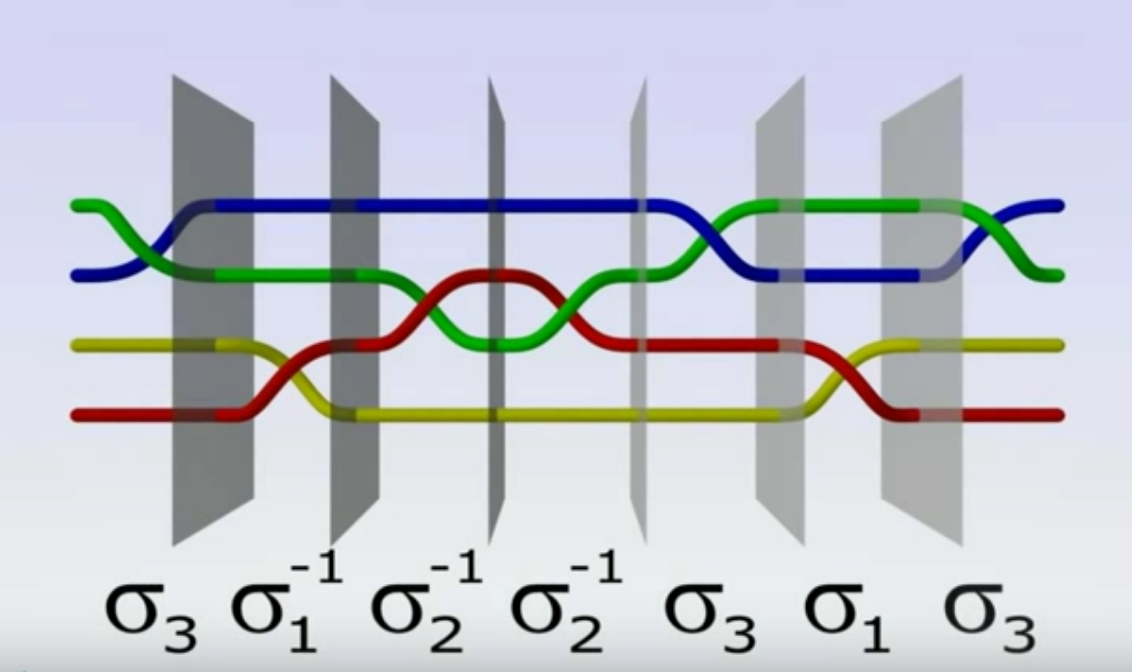
\includegraphics[width=0.6\textwidth]{figures/chapters/2_artin/descomposicion_trenza.png}
    \caption{Ejemplo de composición de trenzas en $B_4$. Fuente: \cite{esterdalvitBraidsChapter12013}}
    \label{fig:elemento_inverso_proceso}
\end{figure}

La secuencia de generadores \(\sigma_3 \sigma_1^{-1} \sigma_2^{-1} \sigma_2^{-1} \sigma_3 \sigma_1 \sigma_3\) en la notación de Artin representa una trenza específica, en la que se aplican cruces de manera secuencial. Esta representación permite visualizar cómo los hilos se entrelazan de acuerdo con las instrucciones dadas por cada generador.

Por ejemplo, como se muestra en la imagen:

\begin{enumerate}
    \item El generador \(\sigma_3\) indica un cruce en el que el hilo 3 pasa sobre el hilo 4.
    \item A continuación, \(\sigma_1^{-1}\) representa un cruce donde el hilo 1 pasa por debajo del hilo 2.
    \item La secuencia \(\sigma_2^{-1} \sigma_2^{-1}\) indica dos cruces consecutivos en los que el hilo 2 pasa por debajo del hilo 3 en cada ocasión.
    \item Luego, \(\sigma_3\) representa otro cruce en el cual el hilo 3 pasa sobre el hilo 4.
    \item Finalmente, los generadores \(\sigma_1\) y \(\sigma_3\) indican cruces adicionales en los que el hilo 1 pasa sobre el hilo 2, y el hilo 3 pasa sobre el hilo 4, respectivamente.
\end{enumerate}

\subsubsection*{Ejemplo de simplificación de una trenza compleja}

Para ilustrar el proceso de simplificación de una trenza compleja utilizando los generadores de Artin y sus propiedades, consideremos la trenza inicial representada por la secuencia:
\[
    \sigma_1 \sigma_3 \sigma_3^{-1} \sigma_2 \sigma_3^{-1}
\]

A continuación, se explican los pasos detallados de simplificación.

\begin{enumerate}
    \item \textbf{Simplificación inicial.} Observamos que en el medio de la secuencia tenemos \(\sigma_3 \sigma_3^{-1}\), que equivale a la trenza identidad. Simplificando, eliminamos esta identidad:
    \[
    \sigma_1 (\sigma_3 \sigma_3^{-1}) \sigma_2 \sigma_3^{-1} = \sigma_1 \sigma_2 \sigma_3^{-1}
    \]

    \begin{figure}[h!]
        \centering
        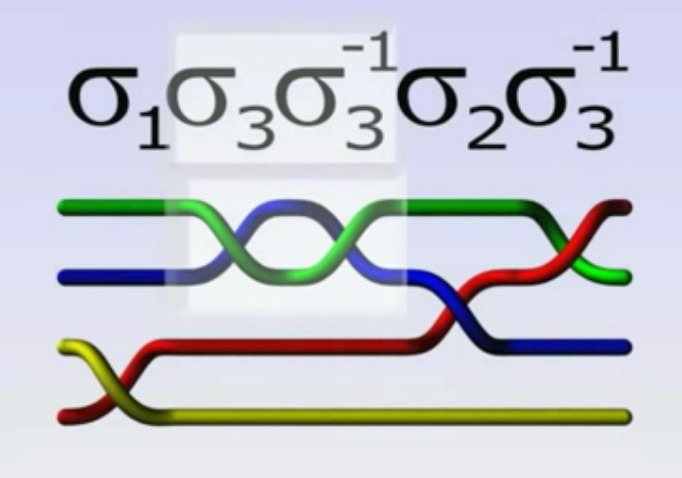
\includegraphics[width=0.3\textwidth]{figures/chapters/2_artin/ejemplo_op_1.png}
        \caption{\cite{esterdalvitBraidsChapter12013}}
    \end{figure}

    \begin{figure}[h!]
        \centering
        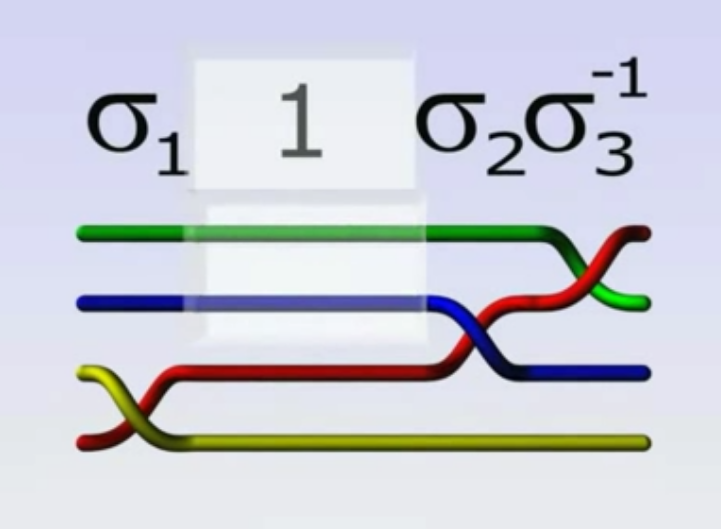
\includegraphics[width=0.3\textwidth]{figures/chapters/2_artin/ejemplo_op_2.png}
        \caption{\cite{esterdalvitBraidsChapter12013}}
    \end{figure}

    \begin{figure}[h!]
        \centering
        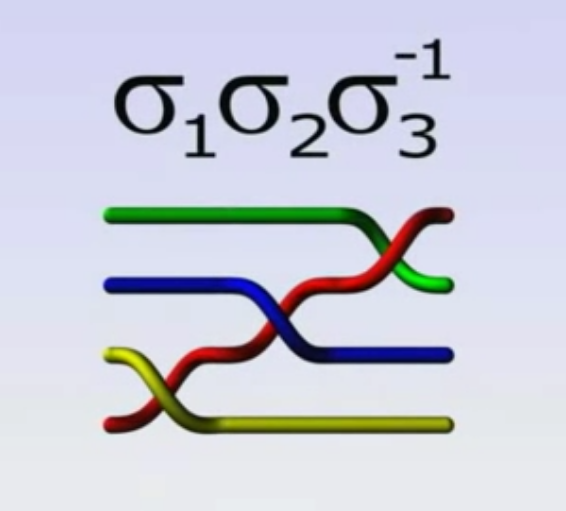
\includegraphics[width=0.3\textwidth]{figures/chapters/2_artin/ejemplo_op_3.png}
        \caption{\cite{esterdalvitBraidsChapter12013}}
    \end{figure}

    \item \textbf{Introducción de trenza adicional.} Para facilitar la simplificación, añadimos la secuencia \(\sigma_2^{-1} \sigma_2\), que también representa la identidad y no afecta la estructura general, pero permite futuras operaciones:
    \[
    \sigma_2^{-1} \sigma_2 \sigma_1 \sigma_2 \sigma_3^{-1}
    \]

    \begin{figure}[h!]
        \centering
        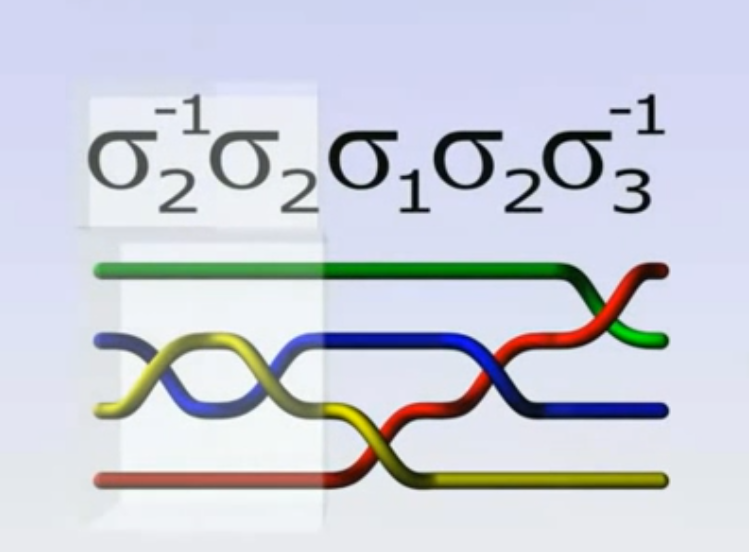
\includegraphics[width=0.3\textwidth]{figures/chapters/2_artin/ejemplo_op_4.png}
        \caption{\cite{esterdalvitBraidsChapter12013}}
    \end{figure}

    \item \textbf{Aplicación de la relación de conmutación en los grupos de trenzas.} Seleccionamos los tres \(\sigma\) del medio (\(\sigma_2 \sigma_1 \sigma_2\)) y los simplificamos utilizando la relación de conmutación en trenzas, que nos permite reordenar esta secuencia como \(\sigma_1 \sigma_2 \sigma_1\). Esto nos lleva a:
    \[
        \sigma_2^{-1} (\sigma_2 \sigma_1 \sigma_2) \sigma_3^{-1} = \sigma_2^{-1} (\sigma_1 \sigma_2 \sigma_1) \sigma_3^{-1}
    \]

    \begin{figure}[h!]
        \centering
        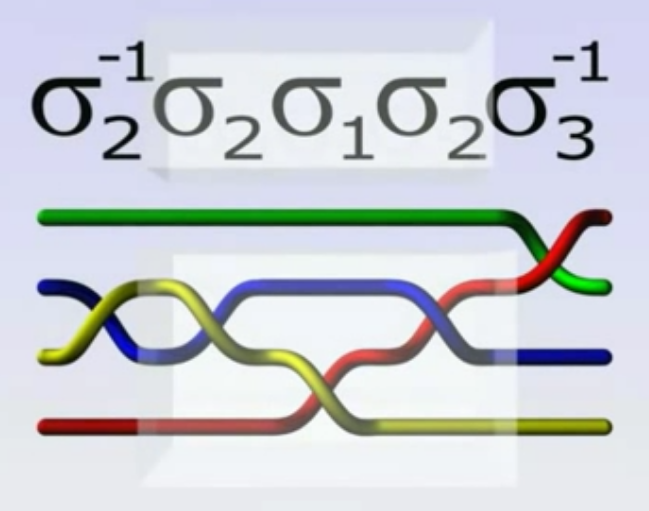
\includegraphics[width=0.3\textwidth]{figures/chapters/2_artin/ejemplo_op_5.png}
        \caption{\cite{esterdalvitBraidsChapter12013}}
    \end{figure}

    \begin{figure}[h!]
        \centering
        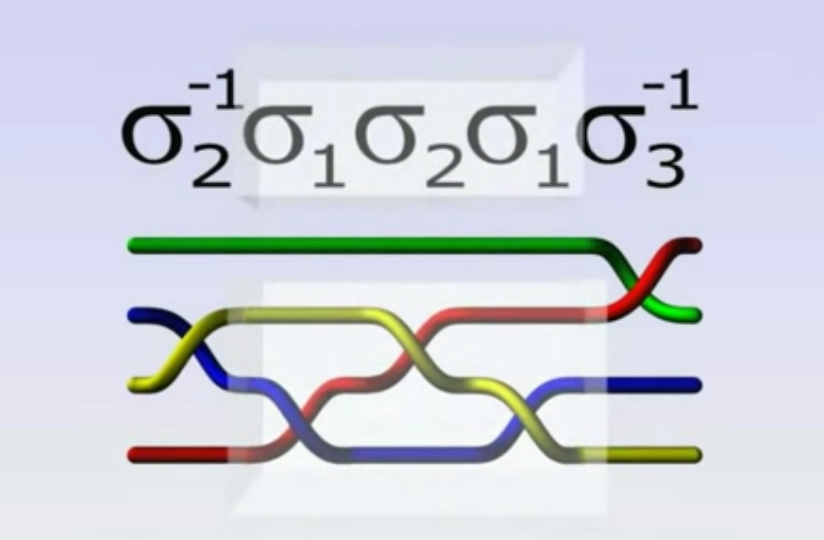
\includegraphics[width=0.3\textwidth]{figures/chapters/2_artin/ejemplo_op_6.png}
        \caption{\cite{esterdalvitBraidsChapter12013}}
    \end{figure}


    \item \textbf{Desplazamiento horizontal de cruces.} Seleccionamos los últimos dos \(\sigma\) (\(\sigma_1 \sigma_3^{-1}\)) y los desplazamos horizontalmente para simplificar la estructura de la trenza, obteniendo:
    \[
        \sigma_2^{-1} \sigma_1 \sigma_2 (\sigma_1 \sigma_3^{-1}) = \sigma_2^{-1} \sigma_1 \sigma_2 (\sigma_3^{-1} \sigma_1)
    \]

    \begin{figure}[h!]
        \centering
        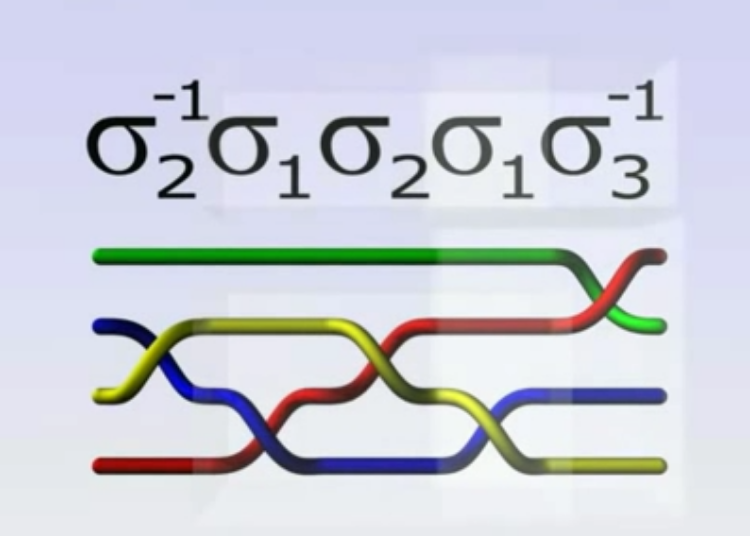
\includegraphics[width=0.3\textwidth]{figures/chapters/2_artin/ejemplo_op_7.png}
        \caption{\cite{esterdalvitBraidsChapter12013}}
        \label{fig:ejemplo_desplazamiento_horizontal}
    \end{figure}

    \begin{figure}[h!]
        \centering
        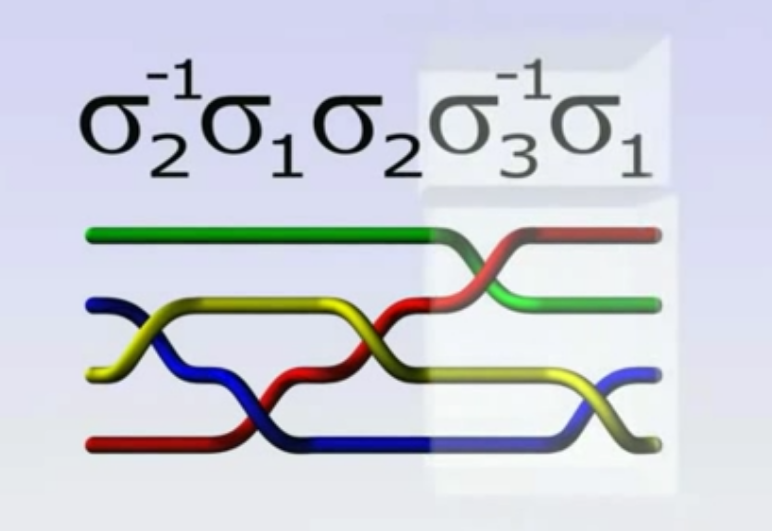
\includegraphics[width=0.3\textwidth]{figures/chapters/2_artin/ejemplo_op_8.png}
        \caption{\cite{esterdalvitBraidsChapter12013}}
    \end{figure}

    \item \textbf{Desplazamiento vertical de la hebra amarilla.} Seleccionamos los tres primeros \(\sigma\) para permitir que la hebra amarilla se desplace hacia abajo, dando como resultado:
    \[
        (\sigma_2^{-1} \sigma_1 \sigma_2) \sigma_3^{-1} \sigma_1 = (\sigma_1 \sigma_2 \sigma_1^{-1}) \sigma_3^{-1} \sigma_1
    \]

    \begin{figure}[h!]
        \centering
        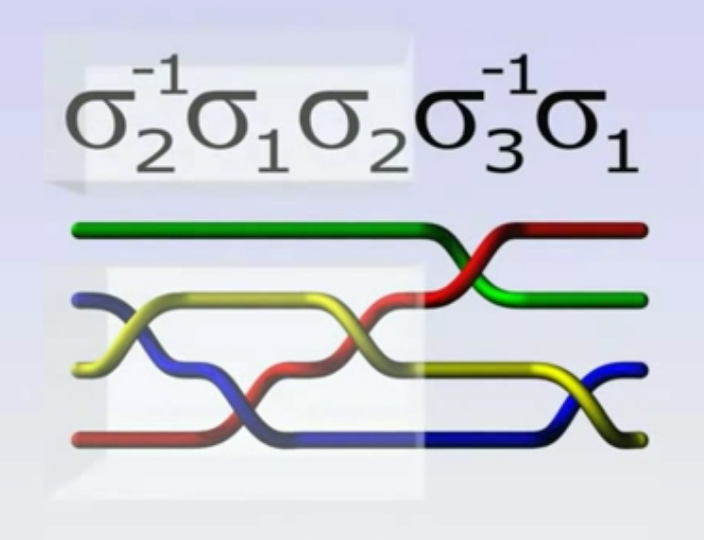
\includegraphics[width=0.3\textwidth]{figures/chapters/2_artin/ejemplo_op_9.png}
        \caption{\cite{esterdalvitBraidsChapter12013}}
        \label{fig:ejemplo_desplazamiento_vertical}
    \end{figure}

    \begin{figure}[h!]
        \centering
        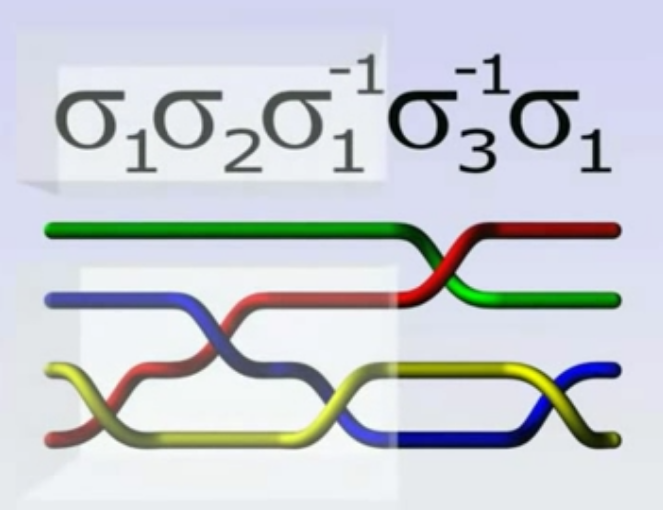
\includegraphics[width=0.3\textwidth]{figures/chapters/2_artin/ejemplo_op_10.png}
        \caption{\cite{esterdalvitBraidsChapter12013}}
    \end{figure}

    \item \textbf{Cancelación de elementos distantes.} Aplicamos una propiedad clave: un generador y su inverso pueden cancelarse aunque estén distantes. En este caso, seleccionamos los tres últimos términos (\(\sigma_1^{-1} \sigma_3^{-1} \sigma_1\)):
    \[
        \sigma_1 \sigma_2 (\sigma_1^{-1} \sigma_3^{-1} \sigma_1) = \sigma_1 \sigma_2 1 \sigma_3^{-1} 1 = \sigma_1 \sigma_2 \sigma_3^{-1}
    \]

    \begin{figure}[h!]
        \centering
        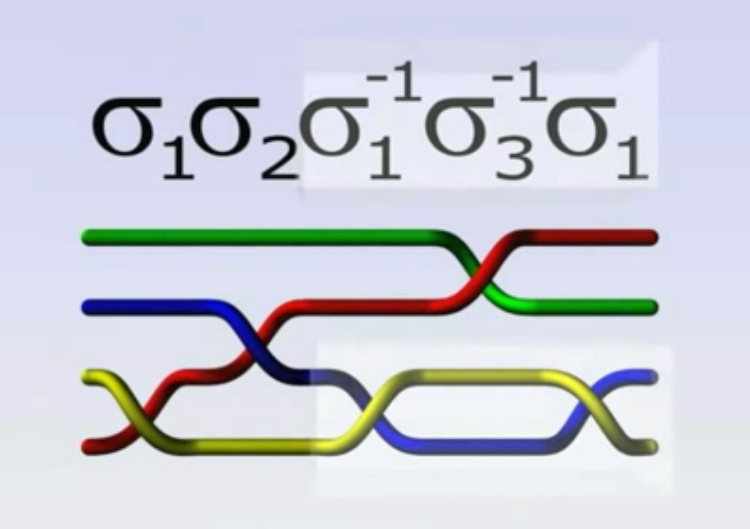
\includegraphics[width=0.3\textwidth]{figures/chapters/2_artin/ejemplo_op_11.png}
        \caption{\cite{esterdalvitBraidsChapter12013}}
    \end{figure}

    \begin{figure}[h!]
        \centering
        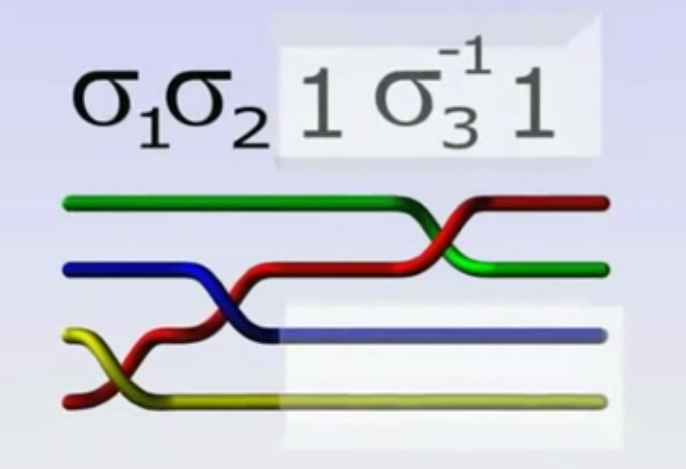
\includegraphics[width=0.3\textwidth]{figures/chapters/2_artin/ejemplo_op_12.png}
        \caption{\cite{esterdalvitBraidsChapter12013}}
    \end{figure}

    \item \textbf{Resultado final.} La secuencia final se reduce a \( \sigma_1 \sigma_2 \sigma_3^{-1}\), representando una trenza simplificada con menos cruces.
\end{enumerate}

Este ejemplo ilustra cómo la aplicación de propiedades fundamentales, como la identidad y la cancelación de elementos, permite simplificar una trenza compleja a una forma más sencilla, facilitando el análisis de su estructura.

% Inverso
\subsubsection*{Ejemplo de operación: Multiplicación de una trenza por su inverso}

\begin{figure}[h!]
    \centering
    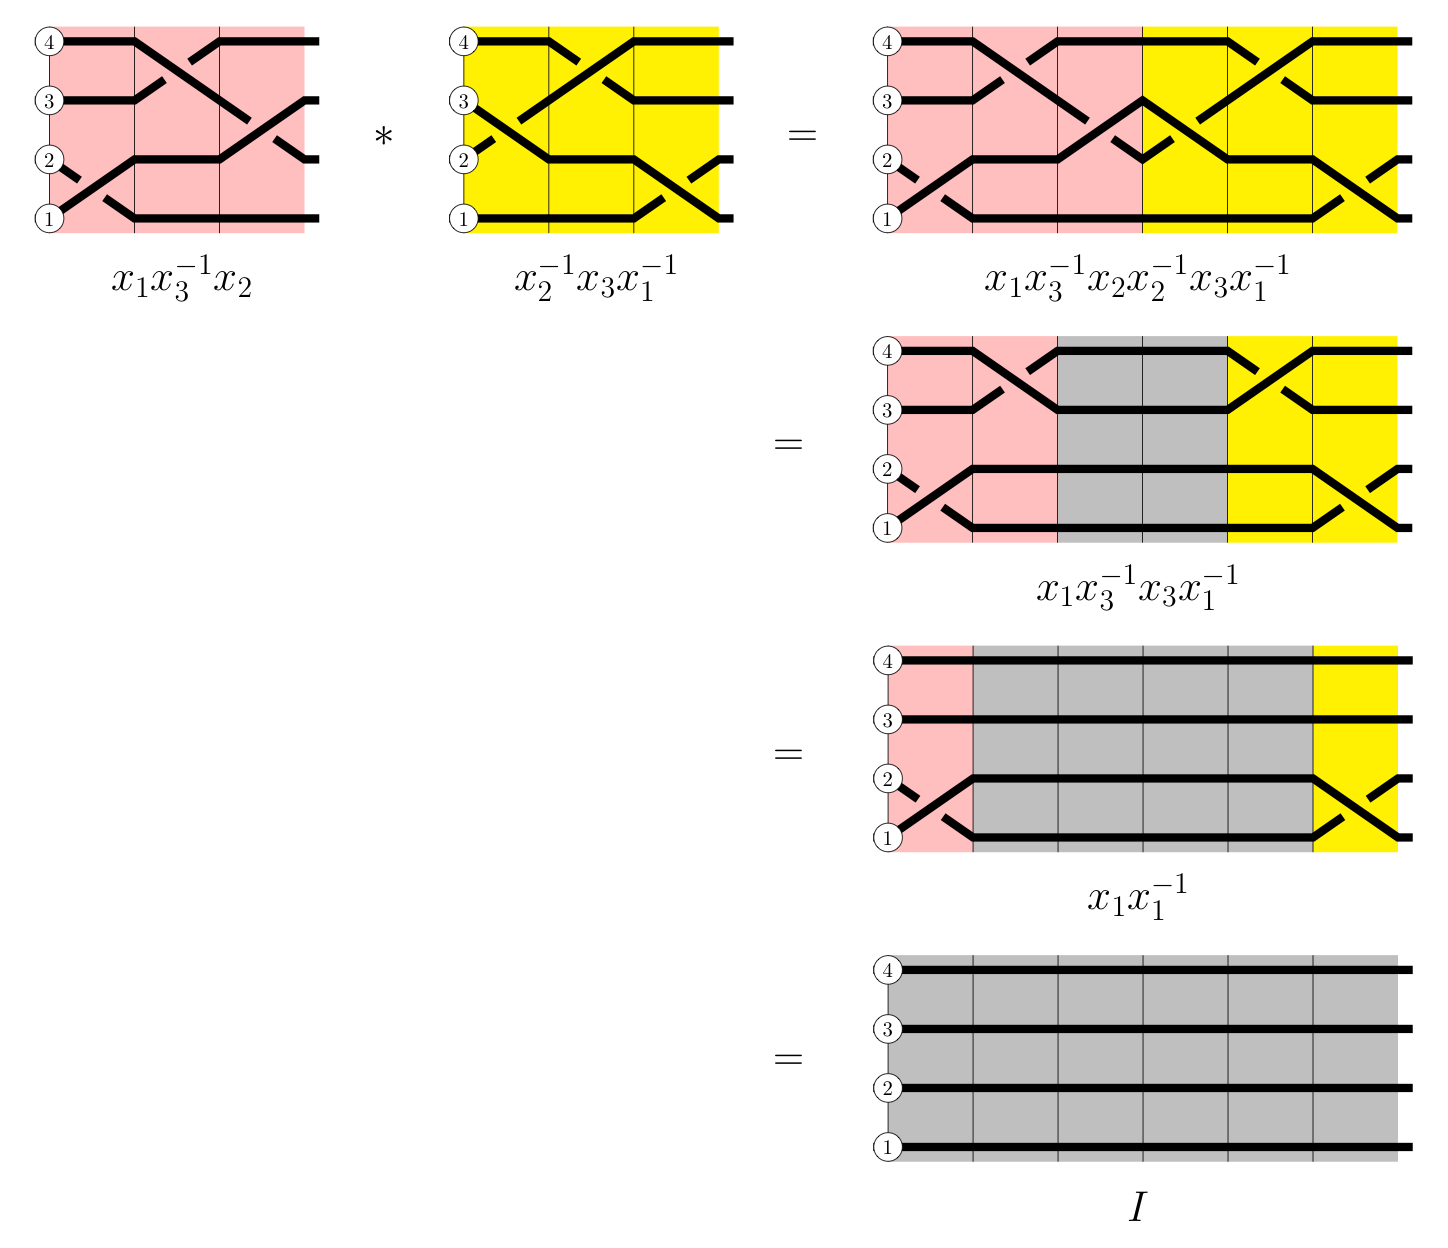
\includegraphics[width=0.6\textwidth]{figures/chapters/1_def_grupo/elemento_inverso2.png}
    \caption{Proceso de operación de un elemento por su inverso en el Grupo de Trenzas $B_4$. Fuente: \cite{ArithmeticBraids}}
    \label{fig:elemento_inverso_proceso}
\end{figure}

En este ejemplo, se muestra cómo multiplicar una trenza compleja por su inverso para obtener la trenza trivial, donde todos los hilos regresan a sus posiciones iniciales sin ningún cruce. La notación utilizada es \(x_i\) para representar el cruce \(\sigma_i\) y \(x_i^{-1}\) para su inverso.

\begin{enumerate}
    \item Comenzamos con una trenza representada por la secuencia de cruces \(x_1 x_3^{-1} x_2\). Esta secuencia indica un conjunto específico de cruces: primero, el hilo 1 cruza sobre el hilo 2, luego el hilo 3 cruza por debajo del hilo 4, y finalmente el hilo 2 cruza sobre el hilo 3.

    \item Para revertir esta configuración, multiplicamos esta trenza por su inverso, representado como \(x_2^{-1} x_3 x_1^{-1}\), de modo que el producto se convierte en:
    \[
    x_1 x_3^{-1} x_2 \cdot x_2^{-1} x_3 x_1^{-1}
    \]
    Este producto representa la trenza original seguida de la secuencia inversa, con lo cual buscamos cancelar los cruces de la configuración inicial paso a paso.

    \item Simplificamos la expresión paso a paso mediante las siguientes operaciones intermedias:
    
    \begin{itemize}
        \item Primero, el cruce \(x_2\) se cancela con \(x_2^{-1}\), resultando en la secuencia \(x_1 x_3^{-1} \cdot x_3 x_1^{-1}\).
        \item Luego, el cruce \(x_3^{-1}\) se cancela con \(x_3\), quedando \(x_1 \cdot x_1^{-1}\).
        \item Finalmente, \(x_1\) se cancela con \(x_1^{-1}\), resultando en la trenza trivial \(I\), donde todos los hilos están en sus posiciones originales sin cruces.
    \end{itemize}

    \item El resultado final es la trenza trivial \(I\), que indica que todos los cruces se han revertido y los hilos han regresado a sus posiciones iniciales. Este proceso demuestra que la multiplicación de una trenza por su inverso da como resultado una configuración sin entrelazado.
\end{enumerate}

Este ejemplo muestra cómo la combinación de una trenza con su inverso permite deshacer los cruces, dejando una estructura en la que los hilos no presentan entrelazado alguno. Esto ilustra la propiedad fundamental de los generadores y sus inversos en la teoría de trenzas.

\newpage

% \subsection{Propiedades fundamentales}

% \begin{itemize}
%     \item \textbf{Localidad}: Cada generador \(\sigma_i\) o \(\sigma_i^{-1}\) afecta únicamente a dos hilos consecutivos, lo cual posibilita la construcción de trenzas de cualquier longitud y complejidad utilizando solo cruces locales.
%     \item \textbf{Asociatividad parcial}: Al combinar varios \(\sigma_i\), el orden de los cruces que no afectan los mismos hilos es irrelevante. Por ejemplo, \(\sigma_1\) y \(\sigma_3\) pueden aplicarse en cualquier orden, ya que no interfieren entre sí.
%     \item \textbf{Existencia de inversos}: Cada cruce \(\sigma_i\) posee un inverso \(\sigma_i^{-1}\), lo cual permite revertir cualquier secuencia de cruces y restablecer la configuración inicial de los hilos.
% \end{itemize}

% En conclusión, la notación de Artin y los generadores \(\sigma_i\) proporcionan una herramienta algebraica para describir y analizar las trenzas, donde cada combinación de cruces define una configuración única de la trenza.

\section{Relaciones de Artin}

\subsection{Teorema 1: Desplazamiento vertical}

El Teorema 1 en la teoría de trenzas describe una propiedad fundamental de los generadores de Artin que permite realizar un desplazamiento vertical de cruces. Esta propiedad se expresa mediante la relación:
\[
\sigma_i \sigma_{i+1} \sigma_i = \sigma_{i+1} \sigma_i \sigma_{i+1}, \quad 1 \leq i \leq n - 2
\]
Esta relación, ilustrada en la Figura \ref{fig:relacion_artin_1}, indica que en un grupo de trenzas, los cruces entre hebras adyacentes pueden reorganizarse manteniendo la equivalencia estructural de la trenza.

Esta propiedad fue utilizada en el ejemplo de simplificación de trenzas en la sección anterior (ver Figura \ref{fig:ejemplo_desplazamiento_vertical}).

\begin{figure}[!h]
    \centering
    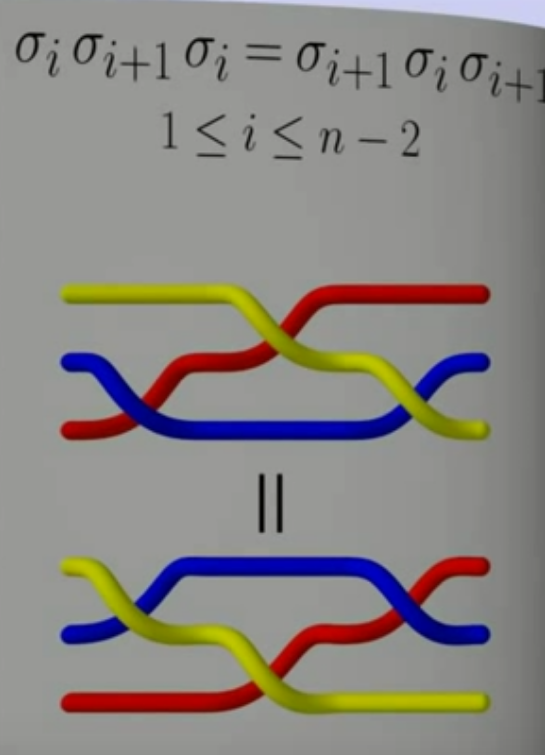
\includegraphics[width=0.4\textwidth]{figures/chapters/2_artin/teorema1.png}
    \caption{Relación de Artin: \(\sigma_i \sigma_{i+1} \sigma_i = \sigma_{i+1} \sigma_i \sigma_{i+1}\). Fuente: \cite{esterdalvitBraidsChapter12013}}
    \label{fig:relacion_artin_1}
\end{figure}

\subsubsection*{Demostración}

Para finalizar, presentaremos una demostración formal del Teorema 1, utilizando las propiedades de las trenzas para justificar cada paso:

\begin{align*}
    x_i^{-1} x_{i+1} x_i &= x_i^{-1} x_{i+1} x_i I \quad &\text{(propiedad de la trenza identidad)} \\
    &= x_i^{-1} x_{i+1} x_i (x_{i+1}^{-1} x_{i+1}) \quad &\text{(uso de trenzas inversas para formar } I\text{)} \\
    &= x_i^{-1} (x_{i+1} x_i x_{i+1}) x_{i+1}^{-1} \quad &\text{(asociatividad de concatenación de trenzas)} \\
    &= x_i^{-1} (x_i x_{i+1} x_i) x_{i+1}^{-1} \quad &\text{(relación de Artin)} \\
    &= \left( x_i x_{i+1} x_i \right) x_{i+1}^{-1} \quad &\text{(asociatividad de concatenación de trenzas)} \\
    &= I x_{i+1} x_i x_{i+1}^{-1} \quad &\text{(cancelación de trenzas inversas)} \\
    &= x_{i+1} x_i x_{i+1}^{-1} \quad &\text{(propiedad de la trenza identidad)}
\end{align*}

Con esta demostración, hemos establecido que el Teorema 1 es válido en los grupos de trenzas, permitiendo el desplazamiento vertical y la reorganización de cruces en configuraciones equivalentes.

\hfill \qed

\newpage

\subsection{Teorema 2: Conmutación de generadores no adyacentes}

El Teorema 2 en la teoría de trenzas establece una propiedad importante de los generadores de Artin, que permite la \textbf{conmutación} de cruces no adyacentes en un grupo de trenzas, lo que se interpreta como un \textbf{desplazamiento horizontal}. Esta propiedad se expresa mediante la relación:
\[
\sigma_i \sigma_j = \sigma_j \sigma_i, \quad |i - j| > 1
\]

Esta relación, ilustrada en la Figura \ref{fig:relacion_artin_2}, muestra que los generadores que actúan sobre hebras no adyacentes pueden intercambiarse sin afectar la estructura global de la trenza. Este desplazamiento horizontal permite reorganizar cruces en distintas posiciones de la trenza sin introducir cambios en su forma general, lo cual es fundamental para la simplificación y manipulación de configuraciones en el grupo de trenzas.

Esta propiedad fue utilizada en el ejemplo de simplificación de trenzas en la sección anterior (ver Figura \ref{fig:ejemplo_desplazamiento_horizontal}).

\begin{figure}[!h]
    \centering
    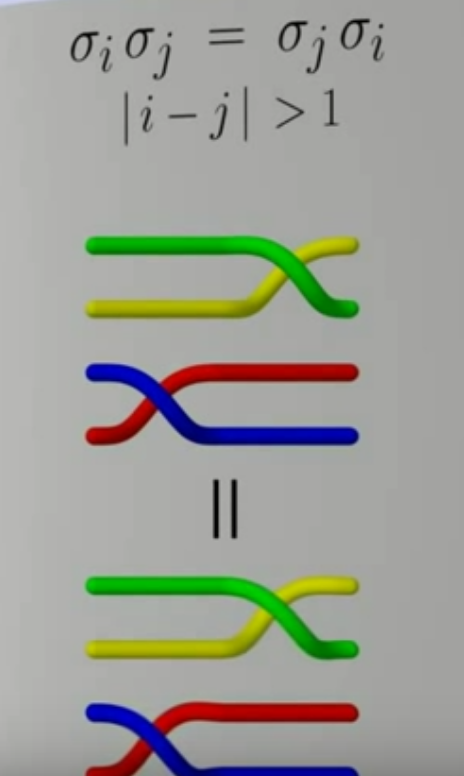
\includegraphics[width=0.4\textwidth]{figures/chapters/2_artin/teorema2.png}
    \caption{Relación de Artin para generadores no adyacentes: \(\sigma_i \sigma_j = \sigma_j \sigma_i\). Fuente: \cite{esterdalvitBraidsChapter12013}}
    \label{fig:relacion_artin_2}
\end{figure}

\subsubsection*{Demostración}

La relación de conmutación para generadores no adyacentes en el grupo de trenzas se demuestra observando que los generadores \(\sigma_i\) y \(\sigma_j\), cuando \(|i - j| > 1\), operan sobre hebras diferentes y no interactúan entre sí. Esto significa que:

\begin{itemize}
    \item El generador \(\sigma_i\) actúa únicamente sobre las hebras \(i\) e \(i+1\), mientras que \(\sigma_j\) actúa sobre las hebras \(j\) y \(j+1\).
    \item Dado que \(|i - j| > 1\), estas hebras son distintas y no comparten ningún cruce o punto de interacción directa entre las hebras \(i, i+1\) y \(j, j+1\).
\end{itemize}

Debido a esta separación, las operaciones representadas por \(\sigma_i\) y \(\sigma_j\) son independientes entre sí, y el orden en que se aplican no afecta la configuración de la trenza. En términos algebraicos, esto implica que:

\[
\sigma_i \sigma_j = \sigma_j \sigma_i
\]

Esta propiedad de conmutación permite reorganizar los generadores no adyacentes sin alterar la estructura general de la trenza, facilitando así la simplificación de expresiones en el grupo de trenzas. La independencia de estos cruces es clave en la teoría de trenzas y refleja que los generadores que actúan en hebras no adyacentes son conmutativos.

\hfill \qed